\documentclass{article}
\usepackage{arxiv} 
\usepackage{graphicx} % Inserting images
\graphicspath{{Images/}} % Expects Image folder in current folder.
\usepackage{float} % Improves h specifier


\usepackage[style=alphabetic]{biblatex}
\addbibresource{references.bib}

\usepackage{amsmath}
\usepackage{amssymb}


\begin{document}
\title{Multidimensional Parameter Decomposition for Mechanistic Interpretability}
\author{Knud Rasmus Sønderbek}
\maketitle
\begin{abstract}
Some super cool abstract of all my findings
\end{abstract}

\section{Introduction}

Mechanistic interpretability seeks to decompose a neural network's
parameters into a set of atoms, each corresponding
to a concrete mechanism underlying the model's computation,
with the goal of simplifying even dense and distributed networks into a simpler, human-interpretable form.


However, both the atomic structure for decomposition
 and the decomposition itself remain open problems.
\autocite{sharkey2025openproblemsmechanisticinterpretability}
Whether a decomposition recovers the computational primitives
of a neural network depends on what the ground-truth decomposition
is taken to be. With models consisting of independent features,
the decomposition is unambiguous, with one atom per feature.
If the features are dependent or co-occur, the decomposition becomes underdetermined.
Decompositions that split features across multiple atoms, risk losing structural information, that gave each feature its meaning,
while decompositions that group multiple features into a single atom, risk losing granularity by collapsing distinct features into a single unit.

For example, a network computing the volume of a cube can be
decomposed into components corresponding to individual side
lengths, or into a single component computing the volume directly.
The former corresponds to a feature-level decomposition,
with one atom per input direction, exposing internal
structure but leaving grouping implicit, only recoverable
through co-activation patterns. The latter corresponds
to a structural-level decomposition, with one atom per
computation, exposing the grouping directly but collapsing per side-length information.

Recently, 
a formal definition of irreducibility was introduced to disambiguate cases such
as the cube example. 
\autocite{engels2025languagemodelfeaturesonedimensionally}
Features are irreducible, and thus constitute units of decomposition,
if their joint distribution cannot be decomposed into independent
factors or into a mixture containing a lower-dimensional component.

In terms of the decomposition itself,
recent work shifts focus from decomposing activations \autocite{sparseautoencoderscanonicalunits} to directly decomposing parameters. Guided by the minimum description length \footnote{not all are but SPD and APD are}, these methods aim to recover components that are faithful to the original weights, sparse per input, and individually simple. 
One such approach, Stochastic Parameter Decomposition (SPD) \autocite{stochasticparameterdecomposition}, factorizes networks into rank-one components with a learned per component importance
function.

This work extends SPD by examining its behaviour on dependent features,
in settings where the multi-dimensional superposition hypothesis posits
a feature-level or a structural-level unit \footnote{I mean feature-level, structure level is wrong under this view but it sounds good} \autocite{engels2025languagemodelfeaturesonedimensionally}. 
Additionally a reformulation of the importance function is proposed,
to encourage that features that are manipulated jointly are grouped together, by computing importance relationally across components.

Findings




\section{Related work}
\subsection{The linear representation hypothesis}
A widespread view in mechanistic interpretability is the linear representation hypothesis: high-level concepts are encoded as directions in a network's representation space \autocite{park2024linearrepresentationhypothesisgeometry}. Together with the superposition hypothesis \autocite{elhage2022toymodelssuperposition}, it forms a central tenet of activation-based interpretability: each feature corresponds to a single direction, and a hidden state is a sparse linear combination of feature directions.

Recent work questions how strictly this view should be taken, distinguishing between a weak form of the hypothesis, that some features are linear, from a stronger form that all features are \autocite{mendel2024sae,smith2024strong}. 
Empirical counterexamples include recurrent networks encoding token position by magnitude rather than direction \autocite{csordás2024recurrentneuralnetworkslearn}, and transformers representing cyclical concepts such as days of the week \autocite{engels2025languagemodelfeaturesonedimensionally} or modular arithmetic \autocite{nanda2023progressmeasuresgrokkingmechanistic} in irreducible low-dimensional subspaces.
\subsection{Activation-space decomposition}
A central direction in activation-based interpretability is the decomposition of learned representations in activation space into interpretable features. An active area of research is the use of 
sparse autoencoders, \autocite{sparseautoencodershighlyinterpretable, bricken2023monosemanticity}
that learn an overcomplete dictionary that expresses each hidden state as a sparse combination of one-dimensional features.
However, these features are not necessarily aligned with the network's computation, due to feature absorption, inconsistencies across dictionary sizes, and a failure to capture feature geometry.
 \autocite{absorptionstudyingfeaturesplitting, sparseautoencoderscanonicalunits,mendel2024sae}.

Circuit discovery extends feature analysis to identify
how a computation is processed through the network's weights
by identifying minimal subgraphs required to maintain
performance on a given task
when the remaining network is ablated \autocite{olah2020zoomin,marks2025sparsefeaturecircuitsdiscovering}.
However, these methods generally do not account for the
polysemantic and densely connected structure of neural networks,
where the functional behaviour can be attributed to multiple distinct but functionally equivalent subgraphs. \autocite{méloux2025everythingeverywhereoncemechanistic}

\subsection{Parameter-space decomposition}

A more recent line of work shifts the object of decomposition from activations to parameters. Transcoders \autocite{dunefsky2024transcodersinterpretablellmfeature} represent an intermediate step that learns a sparse approximation of an MLP layer. Parameter decomposition methods go further, factorising the network's weights directly, with the goal of recovering the network's computational primitives.

Most directly relevant to this work is the description-length-driven
line of Attribution-based Parameter Decomposition
\autocite{AttributionBasedParameterDecomposition} and
Stochastic Parameter Decomposition (SPD)
\autocite{stochasticparameterdecomposition},
recently extended to small transformers
\autocite{christensen2025decompositionsmalltransformermodels}.
While APD decomposes a network into multidimensional
components,
the method is sensitive to hyperparameters, and does not scale beyond toy settings due
to computational complexity. SPD addresses this
by decomposing each weight matrix into rank-one
subcomponents and learning a per-input importance
function over them, at the cost of requiring post-hoc
clustering to recover higher-rank mechanisms;
both methods are detailed in
Section~\ref{sec:spd_background}. Other parameter-space
approaches include local loss landscape decomposition \autocite{chrisman2025identifyingsparselyactivecircuits}.



\section{Method}

\subsection{Background on SPD}
\label{sec:spd_background}
Lukas said to mention apd more + how this did not require the rank 1 constraint, but SPD that is a
solution does
APD issues are computaitonal cost and choosing a hard top k.


This paper builds on the line of work of Attribution-based Parameter Decomposition (APD) \autocite{AttributionBasedParameterDecomposition}
and Stochastic Parameter Decomposition (SPD) \autocite{stochasticparameterdecomposition}, which both aim to decompose
a network's parameters into a set of components that are faithful
to the original weights, minimal in the number required per input,
and individually as simple as possible.

To formalise this, consider a neural network $f(x, W)$ with weight matrices $W = \{W^1, \dots, W^L\}$.
A set of parameter components $\{W^l_c\}_{c=1}^{C}$ are said to comprise the network's mechanisms if they satisfy the following properties:
\renewcommand\labelitemi{\tiny$\bullet$}
\begin{itemize}
    \setlength\itemsep{0em}
    \item \textbf{Faithfulness}: The parameter components should sum to the 
          parameters of the original network.
    \item \textbf{Minimality}: As few parameter components as possible should 
          be required to replicate the network's output on any given input.
    \item \textbf{Simplicity}: Each component should span as few weight 
          matrices and as few ranks as possible.
\end{itemize}

Stochastic Parameter Decomposition (SPD) aims to achieve this by
decomposing the weight matrices of a network
 into a sum of rank-one matrices, called subcomponents:
\begin{equation}
    W^{l}_{i,j} \approx \sum_{c=1}^{C} \vec{U}_{i,c}^{l} \vec{V}_{j,c}^{l}, \quad \text{where} \quad \vec{u} \in \mathbb{R}^{d_{out}}, \vec{v} \in \mathbb{R}^{d_{in}}
\end{equation}
where C is a hyperparameter, for the number of components for each layer, $l$ indexes the layer and $i,j$ are the hidden indices.
The subcomponent count, C, may be chosen to be larger than both $d_{in}$ and $d_{out}$, enabling the method to learn features in superposition \autocite{stochasticparameterdecomposition}.

To enforce the properties above, three losses are introduced, which are optimised jointly.
Faithfulness is enforced thorugh a mean squared error loss between the original network's weights and the the sum of subcomponents:

\begin{equation}
    \mathcal{L}_{\text{faithfulness}} = \frac{1}{N} \sum_{l=1}^{L}\sum_{i,j} \left( W_{i,j}^{l} - \sum_{c=1}^{C} U^{l}_{i,c}V^{l}_{c,j} \right)^{2}  
\end{equation}
where $N$ is the total parameter count in the target model.

Optimization for simplicity and minimality is achieved through a
stochastic masking procedure. Intuitively, if a subcomponent is not
necessary for reconstruction, it can be sampled to zero without loss
of faithfulness. A causal importance function
$\Gamma: \mathcal{X} \to [0,1]^{C \times L}$ is trained to learn the
lower bound of the sampling distribution. In SPD, $\Gamma$ is a set
of independent MLPs $\gamma^l_c$ that each take a layer's activation
and output a scalar importance for the corresponding subcomponent:
\begin{equation}
g^{l}_{c}(x) = \Gamma^l_c(x) = \sigma_{H}(\gamma^{l}_{c}(h^{l}_{c}(x))), \qquad h^{l}_{c}(x) = \vec{V}_{c}^{l\top} \vec{a}^l(x)
\end{equation}
where $\sigma_{H}$ is a hard sigmoid and $\vec{a}^l(x)$ is the
activation at layer $l$. These importance values are used as the lower bound for how much a subcomponent can be masked.
Let $r^l_{c} \sim \mathcal{U}(0, 1)$, then the masked weight matrix becomes
\begin{equation}
\begin{aligned}
    m_{c}^l(x, r) &= g^{l}_{c}(x) + \bigl(1 - g^{l}_{c}(x)\bigr)\, r^l_{c}, \\
    W'^{l}(x, r)  &= \sum_{c=1}^{C} \vec{U}_{i,c}^{l}\, m_{c}^l(x, r)\, \vec{V}_{c,j}^{l},
\end{aligned}
\end{equation}
The training objective becomes that the masked weights should approximately reconstruct the original network's output, with the importance function learning to identify which subcomponents are necessary for reconstruction.
\begin{equation}
    f\!\left(x \,\big|\, \{W'^{l}(x, r)\}_{l=1}^{L}\right)
    \approx
    f\!\left(x \,\big|\, \{W^{l}\}_{l=1}^{L}\right).
\end{equation}
This is done through both a layer-wise and a global reconstruction loss. The layer-wise version is necessary to provide a stronger training signal as randomly masking all components at the same time can be too noisy to learn from.

\begin{equation}
\begin{aligned}
    \mathcal{L}_{\text{stochastic-recon}}
      &= \frac{1}{S} \sum_{s=1}^{S}
         D\!\left(f\bigl(x \mid W'(x, r^{s})\bigr),\; f(x \mid W)\right), \\
    \mathcal{L}_{\text{stochastic-recon-layer}}
      &= \frac{1}{LS} \sum_{l=1}^{L} \sum_{s=1}^{S}
         D\!\left(f\bigl(x \mid W^{1}, \dots, W'^{\,l}(x, r^{(s)}), \dots, W^{L}\bigr),\;
                  f(x \mid W)\right).
\end{aligned}
\end{equation}
where $D$ is a task-specific divergence measure, such as Mean Squared Error for regression tasks or KL divergence.


The masks should also be as sparse as possible, which is enforced by
penalizing the importance values toward zero:
\begin{equation}
    \mathcal{L}_{\text{minimality}}
      = \sum_{l=1}^{L} \sum_{c=1}^{C} \bigl(g^{l}_{c}(x)\bigr)^{p},
      \qquad p > 0.
\end{equation}
\label{spd_minimality}

The full SPD objective is a weighted sum of these terms:
\begin{equation}
    \mathcal{L}_{\text{SPD}}
      = \mathcal{L}_{\text{faithfulness}}
      + \beta_{1}\, \mathcal{L}_{\text{stochastic-recon}}
      + \beta_{2}\, \mathcal{L}_{\text{stochastic-recon-layer}}
      + \beta_{3}\, \mathcal{L}_{\text{minimality}}.
\end{equation}

\subsubsection{Limitations}
Sensitive to hyperparameter minimality loss, 

\subsection{Irreducibility and the natural unit of decomposition}
\label{sec:irreducibility}
To appropriately evaluate the performance of a multi-dimensional feature decomposition method,
it's necessary to have a clear definition of what the ground-truth decomposition is. The original
superposition hypothesis states that the hidden states can be represented as a linear combination of sparse one-dimensional features. \cite{elhage2022toymodelssuperposition,engels2025languagemodelfeaturesonedimensionally} Concretely, the hidden state 
$x_{i,l}$ can be written as:
\begin{equation}
    x_{i,l} = \sum_i v_i \, f_i(t)
\end{equation}
where $v_{i} \in \mathbb{R}^d$ are pairwise $\delta$-orthogonal directions and $f_{i}(t) \in \mathbb{R}$ are sparse scalar activations, with $f_{i}(t)=0$ outside the domain of feature $i$.

Recent work has shown, that this may be insufficiently strict, \autocite{smith2024strong,engels2025languagemodelfeaturesonedimensionally}, as it does not capture the structure of multi-dimensional features.
In particular, transformer models are shown to
organise cyclical concepts in low-dimensional subspaces
that do not decompose into meaningful linear components, but are instead manipulated jointly \autocite{engels2025languagemodelfeaturesonedimensionally}.

To accomodate these features, the same paper proposes a correction to the superposition hypothesis,
alongside a formal definition of irreducibility that defines,
when a feature is in its atomic form and when it can be decomposed into smaller
units without loss of information.

A feature $f \in \mathbb{R}^{d_f}$ is
truly multi-dimensional, if it cannot be written as a sum of two independent features
or as a the sum of two non-co-occurring features. More formally, a feature is
reducible into features
$a$ and $b$ if there exists an affine transformation
\begin{equation}
    f \mapsto Rf + c \equiv \binom{a}{b}
\end{equation}
for some orthonormal $d_{f} \times d_{f}$ matrix $R$, and additive constant c, such that
the joint distribution $p(a, b)$ satisfies one of two conditions:
\renewcommand\labelitemi{\tiny$\bullet$}
\begin{itemize}
    \setlength\itemsep{0em}
    \item \textbf{$p$ is separable}: $p(a, b)= p(a) \, p(b)$
    \item \textbf{$p$ is a mixture of two disjoint distributions}: 
    $p(a, b) = w \, p(a) \, \delta(b) + (1 - w) \, p'(a, b)$,
    with $0 < w < 1$ and $p'(a,b)$ supported on $\{b \neq 0\}$.
\end{itemize}
Here $a$ and $b$ are the first $k$ and remaining $d_f - k$ components of $Rf + c$,
$p$ is conditioned on inputs where $f$ is active, and $\delta$ is the Dirac delta.
In the mixture, the two components have disjoint support: the first lives on the
slice $\{b = 0\}$, a lower-dimensional subspace of the full feature space.

Under this decomposition, the superposition hypothesis takes the form:

Every hidden state $x_{i,l}(t)$ can be written as a sum of feature contributions
\begin{equation}
    x_{i,l}(t) = \sum_i V_i \, f_i(t)
\end{equation}
where each $f_i(t) \in \mathbb{R}^{d_{f_i}}$ is an irreducible
feature with internal dimensionality $d_{f_i} \geq 1$, each
$V_i \in \mathbb{R}^{d \times d_{f_i}}$ and $\| V_i^\top V_j \| < \delta$ for $i \neq j$.

The definition of $V_i \in \mathbb{R}^{d \times d_{f_i}}$ does not require its columns to be linearly independent: $d_{f_i}$ specifies an upper bound on the representational capacity of $V_i$, while $\mathrm{rank}(V_i) \leq d_{f_i}$ determines the effective intrinsic dimensionality required to represent the feature. In practice, this allows models to align dependent components within a shared lower-dimensional subspace (Section \ref{fig:tms-paired-comparison}).
Consequently, features need not correspond to
rank-one directions, but may instead occupy structured subspaces
of higher intrinsic dimension. Decompositions restricted
to rank-one components are therefore not, in general,
aligned with this representation without post-hoc clustering.

\subsection{Rank-$k$ subcomponents and relational importance}
\label{sec:rank-k-attention}
In the original SPD paper, the subcomponents are constructed as rank-one matrices, through an outer product of two vectors.
This formulation is however incompatible with the multi-dimensional superposition hypothesis. (Section \ref{sec:irreducibility})
A decomposition into lower-dimensional subcomponents, necessarily forces features to be split across multiple subcomponents, or to be approximated through a single subcomponent at the cost of reconstruction.

To represent multi-dimensional features, the pairs of vectors are replaced with pairs of matrices.
\begin{equation}
    W^l \approx \sum_{c=1}^{C} U^l_c {V^l_c}^{\top},
    \qquad
    U^l_c \in \mathbb{R}^{d_{\text{out}} \times k},
    \quad
    V^l_c \in \mathbb{R}^{d_{\text{in}} \times k}
\end{equation}
Each subcomponent $U^l_c {V^l_c}^{\top} \in \mathbb{R}^{d_{\text{out}} \times d_{\text{in}}}$
has rank at most $k$, recovering the original SPD definition when $k=1$.
As in the multi-dimensional superposition hypothesis, $k$ is an upper bound on
each subcomponent's representational capacity; the effective rank may be lower,
as it will be discussed \footnote{not a discussion} in Section~\ref{sec:svd_reformulation}.


In SPD, each subcomponent’s importance is computed independently through an MLP followed by a sigmoid nonlinearity,
allowing multiple subcomponents to be active for a given input and thus distribute a
feature across them, even when it is irreducible. Likewise, the minimality loss does not translate to the rank-k setting, where each subcomponent can represent multiple feature directions:
it imposes no penalty for distributing a feature across multiple subcomponents,
nor for a single subcomponent to encode parts of multiple features. (Section \ref{spd_minimality})

To address this, the causal importance function is redefined to maximize the conditional probability, that a given subcomponent c, is responsible for a given feature, conditioned on the activations of all other subcomponents in the same layer.
\begin{equation}
    g^l_c(x) = p\!\left(c \mid \{h^l_{c'}(x)\}^{C}_{c'=1}\right), \quad h^l_c(x) = {V^l_c}^{\top} \vec{a}^l(x) \in \mathbb{R}^k
\end{equation}
where $\vec{a}^l(x)$ is the activation of layer $l$ and C is the set of subcompoennts in layer $l$.
The distribution is computed using a transformer block operating over subcomponents, with a softmax over their activations.


This produces a normalized assignment over subcomponents, $\sum_{c=1}^{C}g^l_c(x) = 1$,
causing the original minimality loss to become degenerate, as each layer contributes a constant value independent of the model state.
Instead, it's replaced
with entropy, to pressure the assignment to concentrate on as few subcomponents as possible. 
\begin{equation}
    \mathcal{L}_{\text{minimality}} = - \frac{1}{|C|} \sum_{l=1}^{L} \sum_{c=1}^{C} g^l_c(x) \log g^l_c(x)
\end{equation}
This pressure is complementary to both the faithfulness loss and the
rank-$k$ extension. If $k$ is too small or the minimality coefficient is too
small, the faithfulness loss dominates and forces features to split across
subcomponents. Conversely, if the minimality weight is too high, the model
groups features together at the cost of faithfulness.

An unfortunate limitation of this formulation is its computational cost. Computing
relational importance via a transformer over subcomponents scales
quadratically with the number of subcomponents compared to the linear cost of the original independent importance functions.  \footnote{Play with attention approximations}

\subsubsection{SVD reformulation, capacity and per feature ablation}
\label{sec:svd_reformulation}
+ add read write streams, theyre a general thing
-> perhaps issues with diffusion and recurrent 
models where this stream is not as clear. https://arxiv.org/pdf/2504.00194
+ add delta orthogonality 

The competition pressure introduced by the softmax has a
theoretical motivation under the multi-dimensional superposition
hypothesis. The hypothesis predicts that different irreducible
features occupy approximately orthogonal projection subspaces;
the softmax-and-attention mechanism implements a training pressure
toward this orthogonality at the level of SPD's atoms. Atoms whose
$V$ matrices share input directions cannot be cleanly distinguished
on inputs that activate those directions, and the softmax
penalises ambiguous allocations. The optimiser's response is to
push the atoms' $V$ matrices toward disjoint subspaces, recovering
the orthogonality structure the hypothesis posits.

Remember to add an experiment that shows if softmax enforce the orthogonality constraint from engels.

\subsubsection{ Per-dimension ablation and implicit rank selection (Hypothesis: ask lukas)}
Following the extension to rank-$k$ subcomponents, and the alternative formulation of the GNAN,
the output $g^{l}_{c} \in [0, 1]^{k}$ is a per feature importance value, and thus the masking can be applied independently to each feature.
The intuition behind this is that if a mechanism captures a 1 dimensional feature, it would only need of the $k$ dimensions to be active.
\\
Likewise if this actually ends up working, k can be considered an upper bound or a so called "capacity" of a mechanism,
it also follows nicely with the descriptive length principle found in the appendix of APD.

To determine the effective rank of each subcomponent, the stochastic masking becomes:
\begin{equation}
    [m_{c}^l(x,r)]_{j} = [g_{c}^l(x)]_{j} + (1-[g_{c}^l(x)]_{j}) r_{c,j}^l, \qquad r_{c,j}^l \sim U(0, 1)
\end{equation}
for each j in $1,\dots,k$
\\
Notably this treats each feature independently, which may not be desirable,
as such we could modify it ever so slightly:

\begin{equation}
        [m_{c}^l(x,r)]_{j} = [g_{c}^l(x)][g_{c}^l(x)]_{j} + (1-[g_{c}^l(x)][g_{c}^l(x)]_{j}) r_{c,j}^l, \qquad r_{c,j}^l \sim U(0, 1)
\end{equation}
The signal becomes an importance of two factors,
if the component is important and both features are important, it remains active,
if only one feature is important, the other will be pushed to zero

The masked weight matrix becomes:
\begin{equation}
    W^{\prime l}(x, r) = \sum_{c=1}^{C} 
    U_{c}^{l} \, \mathrm{diag}\!\left(
    \mathbf{m}_{c}^{l}(x, r)\right) V_{c}^{l\top}
\end{equation}
Where the diagonal matrix is the per-feature mask for subcomponent $c$.

The importance minimality loss penalises all $k$ dimensions of 
all subcomponents toward zero:
\begin{equation}
    \mathcal{L}_{\text{import}} = \sum_{l=1}^{L} \sum_{c=1}^{C} 
    \sum_{j=1}^{k} \left|[g_{c}^{l}(x)]_{j}\right|^{p}
\end{equation}
This follows the same logic by which SPD selects the number of 
active subcomponents: the minimality loss drives unused components 
toward zero, and only those that are genuinely required to 
reconstruct the target model's output survive.

This makes $k$ a soft upper bound rather than a sensitive 
hyperparameter. In practice, $k$ can be set conservatively large 
and the effective rank of each subcomponent is learned from the 
data.




\section{Experiments}
Overview of all experiments, and what they show.
Ive saved an image under images that show how another paper did it.
remember to address the thing in the higher dimensional upscales,
where a clear diagonal is not possible.
\subsection{Reproducing SPD on independent features}
\label{sec:spd-independent-features}
\subsubsection{Sensitivity to hyperparameters}
\label{sec:spd-sensitivity}
\subsection{Softmax without attention}



\subsection{TMS with tied weights and synced inputs}
\label{sec:tms-tied-experiment}



To examine how SPD and the softmax-and-attention extension handle
irreducible features, we reuse the model of superposition introduced
in Section~\ref{sec:spd-independent-features}. The architecture is
a single-hidden-layer autoencoder with tied weights:
\begin{equation}
    f(x) = W^{\top} \sigma(Wx + b), \qquad W \in \mathbb{R}^{d_{\text{hidden}} \times d_{\text{features}}}, \quad d_{\text{features}} \gg d_{\text{hidden}}
\end{equation}
The model is trained to reconstruct sparse feature activations under
an $L_2$ loss. The input distribution differs from
Section~\ref{sec:spd-independent-features} in that features are tied
into pairs. Concretely, $d_{\text{features}} = 40$,
$d_{\text{hidden}} = 10$, and the features are partitioned into
$20$ pairs $\{f_{2i-1}, f_{2i}\}_{i=1}^{20}$. Each pair is zero
with probability $1 - p$, and with probability $p$ both features are
independently drawn from $\mathcal{U} \sim (\epsilon, 1)$.

By construction, the joint distribution of each pair satisfies neither
of the reducibility conditions defined in
Section~\ref{sec:irreducibility}: the activation of one feature in
a pair fully determines the activation of the other, and the joint
distribution has no mass where one feature is zero while
the other is active. By \autocite{engels2025languagemodelfeaturesonedimensionally}, each pair is therefore an irreducible
two-dimensional feature.

Since $d_{\text{features}} \gg d_{\text{hidden}}$, feature representations are necessarily compressed through superposition. In the learned encoder, this results in near-collinearity within feature pairs and approximate orthogonality across pairs.
\begin{table}[h]
\centering
\begin{tabular}{lccc}
\hline
Group        & Mean    & Std Dev & Range \\
\hline
Within-group & $0.999$ & $0.010$ & $[0.997, 1.000]$ \\
Across-group & $0.053$ & $0.223$ & $[-1.000, 0.038]$ \\
\hline
\end{tabular}
\caption{Cosine similarity between encoder columns $W_{:,i}$ and
$W_{:,j}$, partitioned by group membership.}
\label{tab:tms-paired-cosine-similarity}
\end{table}

Under the multi-dimensional superposition hypothesis (Section \ref{sec:irreducibility}),
the formal dimensionality $d_{fi} = 2$, which provides an upper bound on the rank required to represent each feature.
The observed near-collinearity within pairs suggests that this representation essentially collapses to a one-dimensional subspace.

To quantify this, the effective rank of each pair's submatrix, $W_{:,2i-1:2i} \in \mathbb{R}^{d_{\text{hidden}} \times 2}$ is computed using the entropy-based definition of \autocite{effectiverank}.
\begin{equation}
    r_{\text{eff}}(W_g) = \exp\!\left(-\sum_{k=1}^{Q} p_k \log p_k\right),
    \qquad p_k = \frac{\sigma_k^2}{\sum_{j=1}^{Q} \sigma_j^2}
\end{equation}
where $\sigma_k$ are the singular values of $W_g$ and $Q = |g|$.
The quantity lies in $[1, |g|]$ and equals $1$ when the group is
exactly rank-one. To gauge the required value of $k$ for the rank-$k$ extension, the maximum effective rank across pairs is examined:

\begin{equation}
    k = \max_{i} ,\ r_{\text{eff}}(W_{:,2i-1:2i}),
\end{equation}
In this case the max is essentially 1 across all pairs, suggesting that $k=1$ is sufficient to capture these features without loss of information.
(Table~\ref{tbl:mean-effective-rank}).
\begin{table}[h]
\centering
\begin{tabular}{lcc}
\hline
Mean   & Std Dev & Range \\
\hline
$1.0003$ & $0.01$  & $[1.0, 1.05]$ \\
\hline
\end{tabular}
\caption{Effective rank of paired-feature encoder blocks. Values
near $1$ indicate collapse to a single direction.}
\label{tbl:mean-effective-rank}
\end{table}
% Note: numbers are placeholders pending final results.

\subsubsection{Comparison of vanilla SPD and the softmax-and-attention extension}

Both decompositions are trained with $C = 150$ subcomponents and
the hyperparameters proposed in the original SPD paper, with the
exception of the minimality loss, which is set to $x$ for vanilla
SPD and $y$ for the softmax-and-attention extension. We use
$k = 1$, since each pair was shown to be representable along a
single direction in hidden space. The ground truth decomposition is one where each pair is captured by a single subcomponent.


\begin{figure}[H]
    \centering
    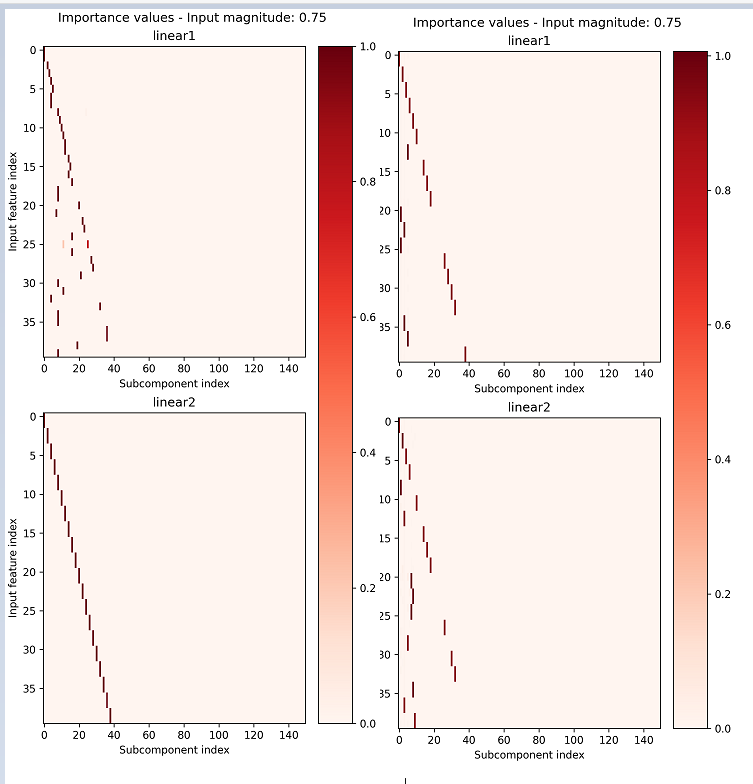
\includegraphics[width=\linewidth, height=15cm]{tms_comparison_rank_1_paired.png}
    \caption{Left: Attention and softmax only at like 15k steps vs 40k steps, Right: Vanilla spd.}
\end{figure}
\label{fig:tms-paired-comparison}

Text explaining what we see, this will change so wait for now.
-Something about if both decompositions are faithful, and if they are faithful to one of the two hypotheses, if they are delta orthogonal, and if the importance values are interpretable.

To verify a successful decomposition, each matrix $V_{i}$ should also be $\delta$-orthogonal to the others.


The multi-dimensional superposition hypothesis predicts that the
projection matrices for different irreducible features are pairwise
$\delta$-orthogonal. At the parameter level, the recovered $V_c$
matrices are the operational counterpart, and the prediction
translates to the requirement that recovered atoms have small
pairwise overlap in their input-side directions.

For each method, we compute the pairwise cosine similarity \footnote{Maybe even UV combined? Only read or write?}
\begin{equation}
    M_{cc'} = \frac{V_c^\top V_{c'}}{\|V_c\| \|V_{c'}\|}
\end{equation}

compared against the across-group cosine similarity of the
trained model's encoder ($0.053$, \ref{tab:tms-paired-cosine-similarity}), the softmax-and-attention shows "something"
and the baseline model finds that "something else".

here we have four nice plots, overall alligment, across V's, across U's, entire thing?
Reference to original model and maybe a table?


% \begin{table}[h]
% \centering
% \begin{tabular}{lcc}
% \toprule
%                            & Vanilla SPD & Softmax-attention \\
% \midrule
% Mean $|M_{cc'}|$ off-diag  & x.xx        & y.yy \\
% Max $|M_{cc'}|$ off-diag   & x.xx        & y.yy \\
% \bottomrule
% \end{tabular}
% \caption{Pairwise overlap of recovered atoms.}
% \end{table}


\textbf{Remarks for this section}
Intra cluster cosine has a -1. Two features are perfectly alligned to a factor of -1,
can this cause issues with decomposition? Same component could capture both features, if they read from the same input.
However they shouldnt as its distinctly different feature indices.



\subsection{Extending to Rank-k: When Higher-Dimensional Structure Matters}
The rank-k extension is required in settings where feature representations do not collapse to a single direction. This is illustrated by a model trained to compute the volume of an n-dimensional simplex.

In this experiment, consider a model trained to compute the volume of an n-dimensional simplex:
\begin{equation}
    f(x) = W_1 \sigma(W_2 x), \quad W_2 \in \mathbb{R}^{k \cdot n(n+1) \times d_{hidden}}, \quad W_1 \in \mathbb{R}^{d_{hidden} \times k}
\end{equation}
Here, k denotes the number of simplices and n the dimensionality of each simplex, which has n+1 vertices.

As in Section~\ref{sec:tms-tied-experiment}, the k simplices are sampled independently with fixed probability, such that either all n(n+1) features of a simplex are active or none are. The resulting feature groups are therefore statistically dependent, and their joint distribution assigns negligible probability to partial activation patterns.
By the definition of irreducibility in Section~\ref{sec:irreducibility}, each simplex constitutes an irreducible feature with formal dimensionality 
$d_{fi}=n(n+1)$.

For this experiment, the model is trained with $n=2$ and $k=4$, yielding four triangles $\mathbb{R}^2$ and a total of 24 input features. The ground-truth decomposition therefore consists of four subcomponents, each responding to 6 adjacent features. 
We note that the effective rank and cosine similarity here imply a decomposition should require at least $k=2$.
\textbf{[Placeholder: cosine similarity results]}

\textbf{[Placeholder: effective rank results, showing $r_{eff} > 1$]}
Firstly, we demonstrate that the original SPD formulation surprisingly yields the best clustered reconstruction when $k=1$:
\begin{figure}[H]
    \centering
    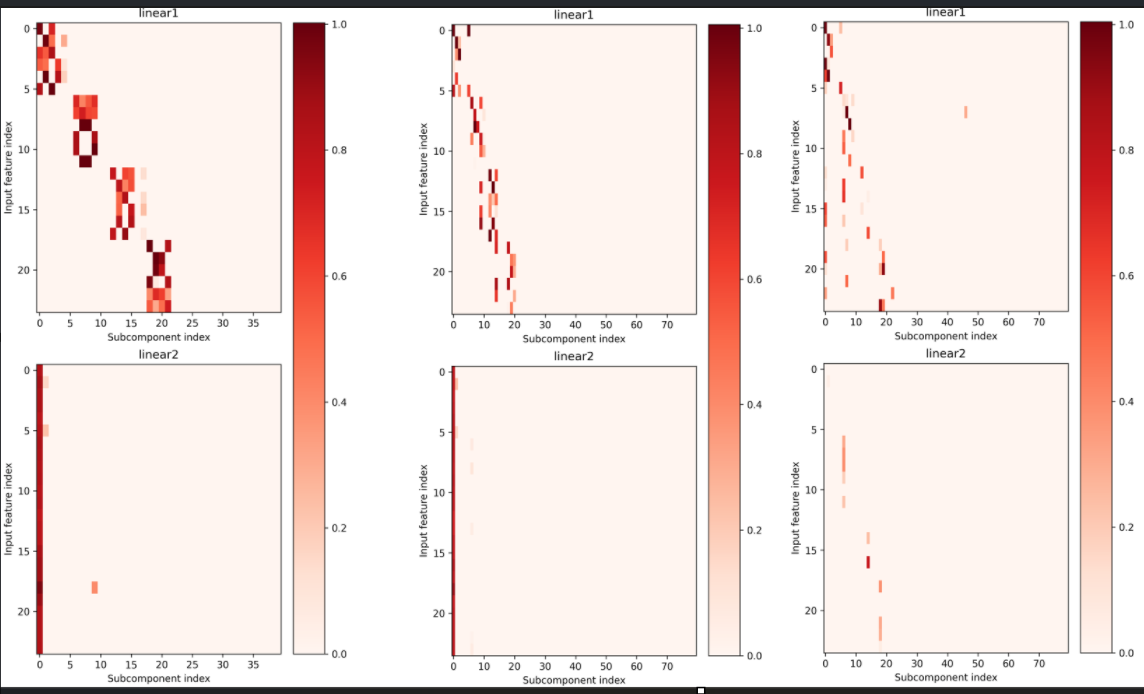
\includegraphics[width=\linewidth, height=8cm]{spd_original_geometry.png}
    \caption{SPD decomposed with k=1,2,3 from left to right.}
\end{figure}
The reconstruction clearly yields 4 subcomponents per group, that only respond to the 6 features of a single simplex, however these subcomponents are seperated even though they are irreducible.

We note that we werent able to find a reconstruction at all when the minimality coefficient was outside of $[1e-4,5e-4]$.

The softmax and attention extension, on the other hand, shows the expected behaviour, with $k=1$, the reconstruction neccessitates that each simplex is split into multiple subcomponents, here each subcomponent captures a single feature.
The extension to $k=2$ allows the model to capture each simplex as a single unit, with all 6 features of a simplex captured by a single subcomponent. However, it does collapse 2 simplices into a single subcomponent. The extension to $k=3$ does not yield any improvement, suggesting that the model has found a faithful reconstruction at $k=2$.
\begin{figure}[H]
    \centering
    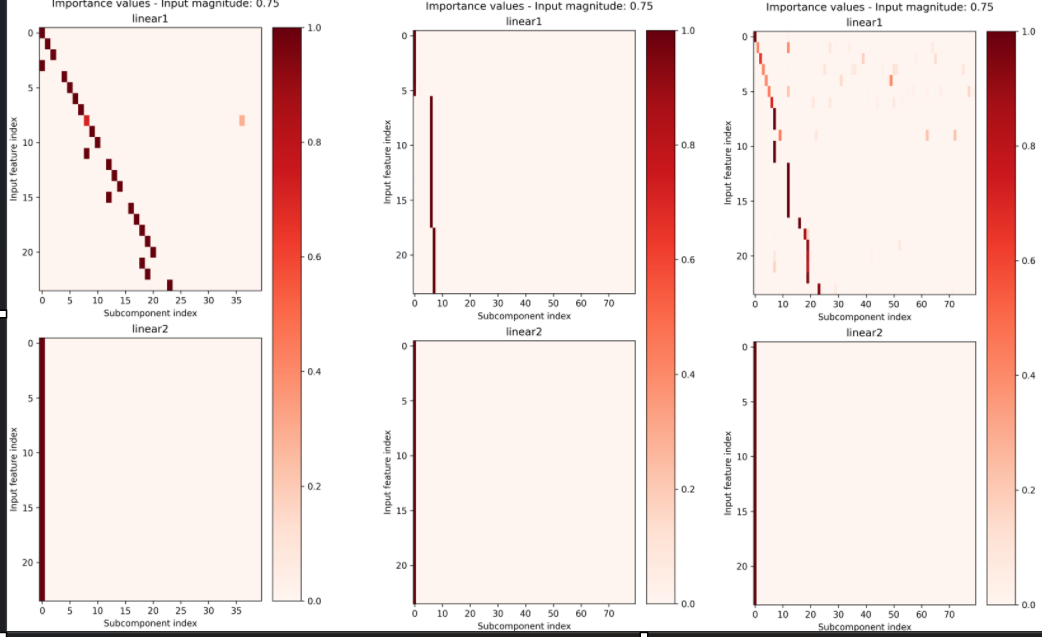
\includegraphics[width=\linewidth, height=8cm]{attention_geometry.png}
    \caption{Softmax-and-Attention decomposed with k=1,2,3 from left to right.}
\end{figure}
While the softmax approach does not find a perfect reconstruction either, it clearly demonstrates how the extension from rank 1 to rank 2 
allows a non diagonal representation of the features. Had it been perfect, then the middle plot would have shown 4 components instead of the collapsed 2.


Same plots i was going to do for the TMS experiment, perhaps this gets its own section,
we compare how input spaces are alligned over training, does the softmax encourage $\delta$ orthogonality better?



\subsection{Checking for orthogonality throughout training with softmax and attention / compare to baseline spd.}

\subsection{Toy model of learning gates}

\textbf{Remark: }
Im not sure we can sample binary values, double check the distribution, i think it requires a continuous thing with b not fixed?
Could always train an addition model, but they already did that in the original paper?
Can we just use that one to prove the claim?



To test the case of enges, where the probability distribution is in fact reducable.
We could train it to learn logic gates i.e
1+0 = 0,
1 + 1 = 1,
0 + 0 = 0,
0 + 1 = 1,
in such a view each could occur independently ,but nlywhen 
both are active, the output is active,
we then sample independently from the two features and see if
it compacts them in a single unit or not.


The concept here is clear:
The ideal decomposition here is one that produces independent features,
that can co occur, however the atomic solution is independence.

We also need to probe for a paired result here. The ground truth should show
part ownership across 2 components.

bool A, bool B are independnet their joint result shoul be shared ownership.


\subsection{Extending the rank to be an upperbound through per feature ablation}




\subsection{Irreducibility as the target of decomposition}

% The methodological extensions developed in the next sections are best
% understood against a formal account of what a faithful decomposition
% of a network with dependent features should recover. \citet{engels2024}
% provide such an account in two parts: a definition of when a feature is
% \emph{irreducible}, and a corresponding hypothesis about how networks
% represent irreducible features in their hidden states.

% \paragraph{Reducibility.}
% A feature $f$ is \emph{reducible} into features $a$ and $b$ if there
% exists an affine transformation $f \mapsto Rf + c \equiv (a, b)$ for
% some orthonormal $d_f \times d_f$ matrix $R$ and constant $c$, such
% that the joint distribution $p(a, b)$ is either separable
% ($p(a, b) = p(a) p(b)$) or a mixture of disjoint distributions ($a$ and
% $b$ are non-co-occurring). A feature is \emph{irreducible} when no such
% decomposition exists.

% Two features that always co-occur, with their joint distribution
% supported on the diagonal $\{(v, v) : v \in \mathcal{V}\}$ together
% with the origin, satisfy neither reducibility condition: the joint is
% not separable (the coordinates are perfectly correlated, not
% independent) and not a disjoint mixture (the coordinates co-occur, not
% exclude each other). Such a pair is therefore irreducible. The paired
% features in the synced-input regime studied in this work are an
% instance of this construction, and the irreducibility framework
% identifies them as a single two-dimensional feature rather than two
% one-dimensional features.

% \paragraph{The multi-dimensional superposition hypothesis.}
% \citet{engels2024} extend the standard superposition hypothesis to
% accommodate irreducible multi-dimensional features. Hidden states are
% written as a sum of feature contributions:
% \begin{equation}
%     x_{i,l}(t) = \sum_i V_i \, f_i(t)
% \end{equation}
% where each feature $f_i(t) \in \mathbb{R}^{d_{f_i}}$ has internal
% dimensionality $d_{f_i} \geq 1$, each projection matrix
% $V_i \in \mathbb{R}^{d \times d_{f_i}}$ embeds the feature into
% hidden space, and the matrices are pairwise $\delta$-orthogonal:
% $\| V_i^\top V_j \| < \delta$ for $i \neq j$. Features are sparse in
% the sense that $f_i(t) = 0$ outside the domain of feature $i$.

% The standard superposition hypothesis is the special case $d_{f_i} = 1$
% for all $i$, in which $V_i$ collapses to a single direction vector.
% The multi-dimensional version is strictly stronger: any feature with
% $d_{f_i} > 1$ can always be expanded as
% \begin{equation}
%     V_i f_i = \sum_{k=1}^{d_{f_i}} V_i^{(k)} f_i^{(k)}
% \end{equation}
% where $V_i^{(k)}$ is the $k$-th column of $V_i$ and $f_i^{(k)}$ is the
% $k$-th coordinate of $f_i$. This expansion fits the form of the
% standard hypothesis but loses the information that the coordinates
% $f_i^{(k)}$ are coordinates of a single irreducible feature rather
% than independent one-dimensional features. The multi-dimensional
% hypothesis preserves this distinction, placing the independence claim
% between whole irreducible features rather than between scalar
% coordinates of unknown irreducibility.

% \paragraph{Implications for parameter decomposition.}
% Hypothesis~2 specifies the granularity at which a faithful
% decomposition should operate: the units of decomposition should be
% irreducible features, with each unit's hidden subspace corresponding
% to a $V_i$ matrix. A decomposition that splits an irreducible feature
% into its scalar coordinates produces units that are not independent
% (they covary according to the irreducible feature's joint
% distribution), and treating them as if they were independent
% misrepresents the model's computation.

% Vanilla SPD operates at the granularity of the standard superposition
% hypothesis: each rank-one subcomponent corresponds to a single
% direction in input space, and there is no mechanism that groups
% subcomponents whose input coordinates are coordinates of a shared
% irreducible feature. Applied to a model representing irreducible
% multi-dimensional features, vanilla SPD therefore recovers
% decompositions whose units are finer than the irreducibility
% boundary. The diagnostic in Section~\ref{sec:vanilla-spd-tms} confirms
% this empirically: on a TMS model trained with paired co-occurring
% features, vanilla SPD assigns one subcomponent per input coordinate,
% splitting each irreducible pair into two atoms.

% The attention extension developed in
% Section~\ref{sec:attention-extension} addresses this gap. By forcing
% subcomponents into competition for assignment to features, the
% extension assigns co-occurring features to a single shared subcomponent
% when the model has internally collapsed them onto a colinear hidden
% representation. The recovered subcomponent's input-side direction $V$
% plays the role of the projection matrix $V_i$ in
% Hypothesis~2\footnote{In the present work the recovered $V$ is
% rank-one rather than $d \times d_{f_i}$. This reflects the fact that,
% when an irreducible feature's joint distribution is fully degenerate
% (the coordinates are perfectly correlated), the model can represent
% the feature using fewer dimensions than its formal internal
% dimensionality $d_{f_i}$ would suggest. The recovered atom matches
% the effective dimensionality the model uses rather than the formal
% $d_{f_i}$, which is appropriate for parameter decomposition: the
% target is faithfulness to the model's representation, not to the
% feature's input-side joint distribution.}, and the recovered atom
% corresponds to the irreducible feature as a single unit.
% \subsection{Atom rank and the effective dimensionality of representations}

% The multi-dimensional superposition hypothesis posits that an
% irreducible feature $f_i$ with internal dimensionality $d_{f_i}$ is
% represented through a projection matrix
% $V_i \in \mathbb{R}^{d \times d_{f_i}}$ embedding the feature into
% a $d_{f_i}$-dimensional subspace of hidden space. The natural reading
% of this hypothesis is that the model uses all $d_{f_i}$ dimensions of
% the available subspace --- that the columns of $V_i$ are linearly
% independent and span a genuinely $d_{f_i}$-dimensional region of
% hidden space.

% This natural reading does not always hold. The model has discretion
% over how much of the available subspace to use, and the joint
% distribution of the feature's internal coordinates determines whether
% this discretion can be exercised without loss of information. When
% the joint distribution is degenerate, the model can represent an
% irreducible feature using fewer than $d_{f_i}$ hidden dimensions while
% still reconstructing the feature's contribution to its outputs
% faithfully.

% \paragraph{An example: perfectly correlated coordinates.}
% Consider an irreducible feature $f_i$ with $d_{f_i} = 2$ whose two
% coordinates are perfectly correlated, taking the same value $v$ when
% the feature is active and zero otherwise. The joint distribution
% $p(f_i^{(1)}, f_i^{(2)})$ has support only on the diagonal
% $\{(v, v) : v \in \mathcal{V}\}$ together with the origin. This
% distribution satisfies neither reducibility condition --- the
% coordinates are not independent (they are perfectly correlated, not
% factorisable) and the joint is not a disjoint mixture (there is no
% regime in which one coordinate varies with the other pinned to zero).
% The feature is therefore irreducible and formally two-dimensional.

% The model representing this feature need not use a full-rank $V_i$.
% Suppose the model chooses
% \begin{equation}
%     V_i = \begin{bmatrix} v & v \end{bmatrix}, \qquad v \in \mathbb{R}^d
% \end{equation}
% in which both columns are the same direction. The contribution of
% this feature to the hidden state is
% \begin{equation}
%     V_i \, f_i = v \cdot f_i^{(1)} + v \cdot f_i^{(2)} = 2v \cdot f_i^{(1)}
% \end{equation}
% where the second equality uses $f_i^{(1)} = f_i^{(2)}$. A single
% hidden dimension is sufficient because the perfect correlation means
% the two coordinates always carry the same scalar value, and the model
% need only track that scalar. The matrix $V_i$ is formally
% $d \times 2$, but its column space is one-dimensional. The feature is
% irreducibly two-dimensional in its input distribution, but the model
% represents it through a rank-deficient $V_i$.

% \paragraph{Effective representational rank.}
% This motivates a distinction between the \emph{formal dimensionality}
% of an irreducible feature, $d_{f_i}$, and the \emph{effective
% representational rank} that the model uses to represent it,
% $\text{rank}(V_i) \leq d_{f_i}$. The two coincide when the feature's
% joint distribution is non-degenerate enough that compression would
% lose information; they come apart when the joint distribution permits
% a lower-rank representation without loss.

% The paired-feature setup studied in
% Section~\ref{sec:paired-experiments} is an instance of the second
% case. The pair is irreducible with $d_{f_i} = 2$, but the trained
% model represents it through a $V_i$ of effective rank one. The
% diagnostic in Section~\ref{sec:diagnostics} confirms this: within-pair
% cosine similarity of the corresponding columns of the model's input
% matrix exceeds $0.99$, indicating that the two columns are
% collinear.

% \paragraph{Implications for atom rank.}
% The required rank of an SPD subcomponent to host an irreducible
% feature as a single unit is the \emph{effective representational rank}
% of that feature in the trained model, not its formal $d_{f_i}$. This
% is at most $d_{f_i}$ but can be less.

% For features the model compresses --- as in the paired case ---
% rank-one subcomponents are sufficient to host the irreducible feature
% as a single unit. The attention extension developed in
% Section~\ref{sec:attention-extension} operates in this regime,
% recovering compressed irreducible features as single rank-one atoms
% whose $V$ aligns with the direction the model uses.

% For features the model represents at full $d_{f_i}$, rank-one
% subcomponents cannot host the feature regardless of additional
% methodological machinery. A simplex feature with non-collinear
% vertices, or a circular feature of the kind \citet{engels2024}
% identify in language models, requires the model to occupy a
% genuinely two-dimensional subspace of hidden space; no compression
% is possible because the joint distribution of vertices does not
% collapse to a one-dimensional locus. Hosting such a feature as a
% single unit requires SPD atoms of rank at least equal to the
% feature's effective representational rank.

% \paragraph{Scope of the present work.}
% The present work develops methods for the compressed regime, where
% the model's effective representational rank is one and rank-one
% atoms suffice. Extending the framework to features the model
% represents at higher effective rank requires SPD atoms with
% rank greater than one, which introduces additional methodological
% considerations beyond the scope of this thesis. The natural next
% direction is the development of rank-$k$ atoms with mechanisms that
% preserve the irreducibility-respecting properties of the present
% method while accommodating features whose representations cannot be
% compressed. This direction is discussed further in
% Section~\ref{sec:future-work}.



\section{Discussion}

\section{Acknowledgements}

\section{References}

\section{Other things to consider?}
Minimal descriptive length?
\subsection{That some features are multidimensional}
Think back to SAE, that learn a dictionary of features,
then find hte linear combination of those features,
however that this fails for cyclical features, as
its cheaper to learn a single feature, than
learn a direction and a periodic function.
Now for your experiment, the dream scenario is that
we allowe a multi dimensional component,
and that this can learn the cyclical feature, i.e a weekly cycle or modular arithmatic
either do this or extend TMS to be multi-dimensional,
show if it works better with ur gnn or not,
likewise we need to show that through individual masking of features,
we can teach a component to kill one of its features,
if it is better explained by a rank 1 component than rank 2.


\section{References}

\printbibliography[heading=none]


\section{Appendix}
Descriptive length thing?

\subsubsection{GNAN-based importance functions}
In SPD, each importance function $\gamma_{c}^{l}$ is an 
independent MLP that receives only its own inner activation. 
Intuitively, however, causal importance is relational: whether 
a subcomponent can be ablated without affecting the output may 
well depend on which other subcomponents are active alongside it.

To address this, the independent MLPs are replaced with a Graph Neural Additive Network (GNAN)
that can relate each subcomponent to its neighbourhood.

The $C$ subcomponents are treated as nodes in a graph, with node 
features given by their inner activation vectors 
$\mathbf{h}_{c}^{l}(x) \in \mathbb{R}^{k}$. The GNAN updates 
each node's representation through an additive neighbourhood 
aggregation. For node $i$ in layer $l$ and feature dimension $k$ \footnote{I am very open to alternative equations, i.e perhaps we delete the layer distance inside rho, however it seemed necessary to use cosine similarity, as otherwise the signal was useless as described in some earlier section}:
\begin{equation}
    [\mathbf{z}_{i}]_{k} = \sum_{j=1}^{N} 
    \frac{1}{|\mathcal{L}(j)|} \cdot 
   \rho\!\left(\frac{1}{1 + \mathrm{dist}(j, i)},\; 
\mathrm{cos}(j, i)\right) \cdot 
    f_{k}\!\left([\mathbf{h}_{j}]_{k}\right)
\end{equation}
OBS: Implementation ill present today is this:

\begin{equation}
    \mathbf{z}_{i} = \sum_{j=1}^{N} \rho \left( \text{layer distance}, \text{cosine similarity} \right) \cdot f_{k}\left( [\mathbf{h}_{j}]_{k} \right)
\end{equation}
where $f_{k}$ is a learned function applied to the $k$-th inner 
activation of each neighbouring node $j$; $|\mathcal{L}(j)|$ is 
the number of nodes in the same layer as $j$, which normalises 
the contribution of each 
layer; $\mathrm{dist}(j, i)$ is the layer distance between 
nodes $j$ and $i$\footnote{The layer distance, could later be signed to differentiate between
previous and future layers}; $\mathrm{cos}(j, i)$ is the cosine similarity 
between their parameter vectors; and $\rho$ is a learned function 
that maps both the distance kernel and the cosine similarity to a 
scalar weight.

$z_{i}$ becomes a vector in $\mathbb{R}^{k}$, which 
fits perfectly with the current activation vectors.

A separate MLP is trained to combine the aggregated neighbourhood information and the node's own activation into an importance value in $[0, 1]$:
Producing a single importance value per subcomponent and passing it through 
a leaky hard sigmoid, following 
SPD \autocite{stochasticparameterdecomposition}:
\begin{equation}
   g_{c}^{l} = \sigma_{H}(AGG(\mathbf{z}_{i}^l, \mathbf{h}_{i}^l))
\end{equation}
The self-connection through $f_{\text{self}}$ (or just the raw activation) ensures that each 
node retains its own identity after aggregation, mitigating 
the oversmoothing that can occur in GNNs. \{Clever cite here, i.e gnn book\}


\textbf{Alternative formulation, that would work with the next section} \\

After the GNAN update, the per-dimension importance values are 
computed from the updated representation and passed through a 
leaky hard sigmoid, following 
SPD \autocite{stochasticparameterdecomposition}:
\begin{equation}
    \mathbf{g}_{c}^{l}(x) = \sigma_{H}\!\left(\mathbf{h}_{c}^{l}(x)\right)
    \in [0, 1]^{k}
\end{equation}
in other words, the importance function becomes multidimensional,
and each column can be masked independently.

\textbf{Remarks:} \\
For now the edge set construction is left as the fully connected graph,
which remains reasonably computationally expensive for small models.
However it could very easily be made more efficient, for other architectures,
or by considering only the k-hop neighbourhood of each node, or only considering prior neighbours or later neighbourhoods.
Likewise we could store both distances as sparse structures as they are symmetric. $\cos (j,i) = \cos (i,j)$
\\
\textbf{Remark 2:} \\
The choice of edge set construction and distance function is a very important design choice,
e.g using the layer distance on a fully connected graph encodes the same signal for all nods in a layer:
For nodes $i_1, i_2$ in the same layer $l$:
\begin{equation}
    \forall\, j \colon \quad 
    \mathrm{dist}(j, i_1) = \mathrm{dist}(j, i_2) = |k_j - l|
\end{equation}
and therefore
\begin{equation}
    [\mathbf{h}_{i_1}]_k = \sum_{j=1}^{N} 
    \frac{1}{\#\mathrm{dist}_{i_1}(j, i_1)} \cdot 
    \rho\!\left(\frac{1}{1 + |k_j - l|}\right) \cdot 
    f_k([\mathbf{x}_j]_k) 
    = [\mathbf{h}_{i_2}]_k
\end{equation}
since no term in the sum depends on the identity of $i$ 
within layer $l$, only on the layer index $l$ itself.
\\
Additionally this produces a counterproductive signal,
the gnan tries to boost or suppress all nodes in a layer together, instead
of learning to differentiate between them.

\textbf{Remark 3:} \\
The choice of distance should probably be reconsidered in general,
I have a feeling that the function needs to be from an asymmetric metric space,
i.e
\begin{equation}
    dist(i, j) \neq dist(j, i)    
\end{equation}
Atleast if the intution is if component A in layer k, is highly active, perhaps component B in layer
k+1 should likely be inactive, as the other component needs to handle this feature,
thus the distance from A to B should be different, as otherwise both are boosted or suppressed together. 

\textbf{Remark 4:} \\
The current experiments are more sensitive to hyperparameters,
than the original code seems to be, if the minimality pressure is too low, then all components are active, and doesn't "kill" any of them

\textbf{Remark 5:} \\
I haven't been able to find any "benefit" in setting k higher,
this is ofcourse because hte ground truth of all the models we have
are rank 1 independent features, we need to find a scenario where the dependence and or rank k is actually necessary:

My ideas
\renewcommand\labelitemi{\tiny$\bullet$}
\begin{itemize}
    \setlength\itemsep{0em}
    \item Sample points from the unit circle, i.e $\cos(\theta)^2+ \sin(\theta)^2 = 1$ then
    \begin{align*}
        x = \sqrt{1-\sin (\theta)^2} \text{ or} -\sqrt{1-\sin(\theta)^2} \\
    \end{align*}
    i.e sometihng can only be expressed with a rank 2 component?
    \item we could look for circuits, the goal is then no longer to find N independent features, but suppose we have input groups [0,1,2], [2,3,4], [3,4,5] then we want one component that activates for the first group, one for the second and one for the third
\end{itemize}

\textbf{Remark 6:} \\
I added the gnan plots to wandB remember to show them

\textbf{Remark 7:} \\
The per feature construction with only 1 feature is rather boring, and does not utilize the expressiveness at all.

\textbf{Remark 8:} \\
I dont think its a code problem,
as i can reproduce equivalent results to their findings.
Im just not able to beat them.
We need to discuss experiments where the k dimensionality and dependence
actually matters.



\section{ Old Introduction - may be useful for related work.}


Neural networks continue to achieve remarkable performance across domains ranging from medical diagnosis to
autonomous systems. This increase in performance has, however,
come with a corresponding increase in complexity, making these systems
less interpretable to those who build and deploy them.
As neural networks enter high-stakes environments,
where errors carry legal, financial, or human cost, interpretability becomes a necessity. The concern is not merely technical but ethical: a fundamental principle of accountability holds that the creator of a tool can only be held responsible for its outcomes to the extent that those outcomes could have been reasonably foreseen.
A system whose internal reasoning cannot be understood is, by definition,
one whose failures cannot be anticipated.

Mechanistic interpretability aims to reverse-engineer the internal computations
of neural networks into their simplest forms, such that they can be expressed as humanly interpretable
algorithms.\\
Many of the current popular methods within this space, such as sparse autoencoders \cite{sparseautoencodershighlyinterpretable},
circuit analysis, and probing, primarily operate in activation space.
However, each of these methods comes with its own set of limitations.
Sparse autoencoders treat features as independent directions and discard
the geometric structure between them,
despite growing evidence that this structure carries meaningful information
(Leask et al., 2025; Mendel, 2024; Engels et al., 2024). 
Moreover, sparse autoencoders are trained to reconstruct activations and do not to explicitly identify the computational units that produced them. \cite{sparseautoencoderscanonicalunits, absorptionstudyingfeaturesplitting}
The resulting decomposition may be functionally equivalent at a given layer, while
not resembling the mechanisms that the network employs.
Circuit-level methods face the deeper issue that neural networks are densely connected,
meaning any given output can be equally well attributed to a multitude of causal pathways, leaving the choice of circuit underdetermined.

A more recent line of work aims to decompose the parameters of the network directly, rather than the activations.
More concretely, these methods aim to decompose a network's weights into a sum of simpler components, 
each of which corresponds to a concrete "mechanism". This reframing sidesteps several of the issues above:
mechanisms are no longer constrained to specific architectural components, such as neurons or attention heads,
and can instead be distributed across multiple architectural components. Moreover,
they decompose the network into functional units rather than representational directions,
which may further enhance their interpretability.
\\
Recently proposed methods guided by the principle of minimum description
length have shown promising results in this direction, aiming to decompose a network
into parameter components that are faithful to the original weights, minimal in the number
required per input, and individually as simple as possible.
\\
One such method, Stochastic Parameter Decomposition (Bushnaq et al., 2025), decomposes networks into rank-one subcomponents. Since not all components are relevant for every input, the method learns a function that estimates each component's causal importance for a given input. However, each component's importance is calculated independently, relying only on its own activation. As noted in the original work, this is likely too restrictive for non-toy models, as it prevents each component's importance from being informed by the state of other components. This work replaces the independent importance functions with a graph neural network that determines each component's importance conditioned on its relationships to all other components, while preserving explainability through its generalised additive structure.
Additionally the use of an additive importance function, generalizes the decomposition to k-dimensional components.
This generalizsation is motivated by the growing evidence, that transformer models, learn features
which occupy irreducible multidimensional subspaces.


\section{Notes}
Putting the minimality lsos entropy higher, encourages diagonals?
Instead of capturing two features in the same component.

Increasing minimality loss encourages feature grouping.

SAE: learn to decompose activations, i.e the output of a layer,
Transcoders: learn to approximate the input-output function of a layer



\[
\int p(a,b)\,da\,db
= w \int p_A(a)\,da \int \delta(b)\,db
+ (1-w)\int\!\!\int p_{AB}(a,b)\,da\,db
= w + (1-w)
= 1
\]

to read:
Terence Tao, \emph{An Introduction to Measure Theory}:
Section 1.1 Prologue: The problem of measure --- sets up why measure theory exists and why "lower-dimensional sets have measure zero" is the central idea. This alone might give you the intuition you need.
Section 1.2 Lebesgue measure --- gives you "measure zero," "Lebesgue measure on $\mathbb{R}^n$," and the fact that lines/planes/etc. have measure zero in higher-dimensional ambient spaces. This is the technical core for your question.
Section 2.3 Probability spaces --- short section that frames everything in probability language, which is what you actually want.
\end{document}